\documentclass[conference]{IEEEtran}
\usepackage{amsmath,amssymb}
\usepackage{booktabs}
\usepackage{array}
\usepackage{url}
\usepackage[hidelinks]{hyperref}
\usepackage{microtype}
\usepackage{pgfplots}
\pgfplotsset{compat=1.18}
\usetikzlibrary{positioning,arrows.meta}
\newcolumntype{L}[1]{>{\raggedright\arraybackslash}p{#1}}

\begin{document}

\title{Multi-Backbone SED Ensembles with Snippet-Bank Matching for Indic Noise Event Detection}

\author{\IEEEauthorblockN{Shivam Dwivedi, Animish Yadav, Shubhi Jain}
\IEEEauthorblockA{Team TDS, Indraprastha Institute of Information Technology Delhi (IIIT Delhi), India\\
\{shivam21352, animish23089, shubhi23517\}@iiitd.ac.in}}

\maketitle

\begin{abstract}
We describe our Track~1 system for the Datathon@IndoML~2026 noise event detection challenge: localising
class-agnostic onset/offset pairs of noise events in Indic speech from the Vaani corpus, scored by event F1 plus
segment Dice~\cite{metrics}. The system combines (i) an ensemble of twelve frame-level sound event detectors built
on five pretrained encoders (ATST-F, BEATs, WavLM-base+/large, w2v-BERT~2.0), each fused with a mel-CNN and a
BiGRU emitting 24 presence and boundary tracks; (ii) a \emph{snippet bank}: the organizers' synthetic mixtures
reuse sample-exact noise snippets, which we isolate from validation pairs and detect with calibrated matched
filtering; and (iii) a routing decoder, tuned under test-mixture weighting, that merges bank and neural evidence
per clip. Our final submission (Codabench 995227) reaches event F1 0.7711 and segment Dice 0.8232, a combined score
of 1.5943 (rank~6), up from 1.2129 for our Phase~1 entry.
\end{abstract}

\begin{IEEEkeywords}
sound event detection, ensembles, self-supervised encoders, matched filtering, Indic speech
\end{IEEEkeywords}

\section{Training Data and Preprocessing}
\subsection{Data sources}
Table~\ref{tab:data} lists the data. No external datasets are used beyond the pretrained encoders of
Table~\ref{tab:pre}. The \textbf{IndoML validation set} is split into five folds; fold~4 (479 clips: 344 natural,
135 synthetic) is the monitor and selection hold-out and is never trained on.

\begin{table}[b]
\centering
\caption{Training data. Vaani tiers follow the dataset's annotation quality.}
\label{tab:data}
\footnotesize
\setlength{\tabcolsep}{3pt}
\begin{tabular}{L{2.5cm}L{2.0cm}L{3.1cm}}
\toprule
Source & Size & Use\\
\midrule
Vaani~\cite{vaani} Gold (verified timestamps) & 11,111 seg., 21.8\,h & frame targets; noise events and speech for
mixtures\\
Vaani Silver (unverified timestamps) & 61,642 seg., 100.3\,h & frame targets (down-weighted)\\
Vaani Bronze (tags only) & 17,884 seg., 32.4\,h & multiple-instance (MIL) clip head\\
IndoML validation, natural, folds 0--3 & 1,462 clips & extra frame targets for six members\\
IndoML validation, synthetic & 695 pairs & snippet bank (206 snippets); clean speech for mixtures\\
\bottomrule
\end{tabular}
\end{table}

\subsection{Targets and synthetic mixtures}
Each clip yields 24 channels at a 20\,ms frame rate: union presence, seven category presence tracks, and union plus
per-category onset/offset tracks (Gaussian boundary targets). The organizers' synthetic clips are built as
$\text{noisy}=\text{clean}+\sum_i g_i\,\text{snippet}_i$ with labels exact to the sample. We regenerate such
mixtures on the fly, using event counts, gaps ($\geq$200\,ms), gains and durations measured on the 695 validation
synthetic clips. Noise comes from the snippet bank and, for widened members, isolated Gold event spans; speech comes
from validation clean references (held-out folds excluded) and Gold/Silver speech regions at least 50\,ms from any
event.

\subsection{Batches and augmentation}
Batches mix the sources in fixed proportions (e.g.\ Gold 0.40, Silver 0.27, Bronze 0.05, synthetic 0.28). Crops are
event-biased: 80\% contain a whole event and 10\% are hard negatives, with 10\,s crops (4\,s for the breath
specialist). Augmentations are random gain, label-preserving whole-frame time shifts, label-union mixup within a
tier, FilterAugment~\cite{filteraug} band gains, and optional Freq-MixStyle.

\section{Proposed Method}
\begin{figure}[t]
\centering
\resizebox{\columnwidth}{!}{%
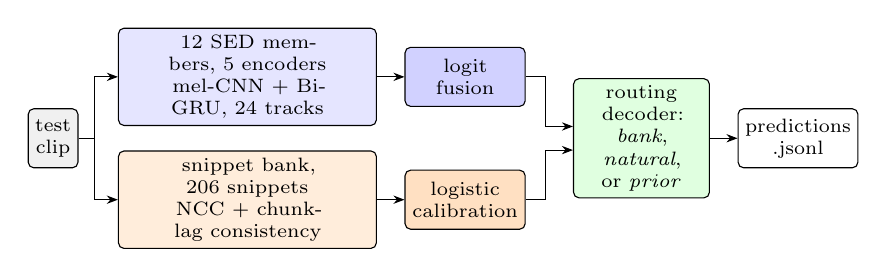
\begin{tikzpicture}[font=\scriptsize, >={Stealth[length=4pt]}, node distance=0.4cm,
  blk/.style={draw, rounded corners=2pt, align=center, minimum height=0.75cm, inner sep=2.5pt, fill=#1},
  blk/.default=white]
\node[blk=gray!12] (x) {test\\clip};
\node[blk=blue!10, text width=3.1cm, right=0.5cm of x, yshift=0.78cm] (sed)
  {12 SED members, 5 encoders\\mel-CNN + BiGRU, 24 tracks};
\node[blk=blue!18, text width=1.35cm, right=0.35cm of sed] (fus) {logit fusion};
\node[blk=orange!14, text width=3.1cm, right=0.5cm of x, yshift=-0.78cm] (bank)
  {snippet bank, 206 snippets\\NCC + chunk-lag consistency};
\node[blk=orange!24, text width=1.35cm, right=0.35cm of bank] (cal) {logistic calibration};
\node[blk=green!12, text width=1.55cm, right=0.6cm of fus.east, yshift=-0.78cm, anchor=west] (route)
  {routing decoder:\\\emph{bank},\\\emph{natural},\\or \emph{prior}};
\node[blk, right=0.35cm of route] (out) {predictions\\.jsonl};
\draw[->] (x.east) -- ++(0.2,0) |- (sed.west);
\draw[->] (x.east) -- ++(0.2,0) |- (bank.west);
\draw[->] (sed) -- (fus);
\draw[->] (bank) -- (cal);
\draw[->] (fus.east) -- ++(0.25,0) |- ([yshift=0.15cm]route.west);
\draw[->] (cal.east) -- ++(0.25,0) |- ([yshift=-0.15cm]route.west);
\draw[->] (route) -- (out);
\end{tikzpicture}}
\caption{System overview. Fused neural probabilities and calibrated bank matches meet in a per-clip routing
decoder; every clip receives at least one event.}
\label{fig:arch}
\end{figure}

\subsection{Neural SED members}
Each member (Fig.~\ref{fig:arch}) fuses a pretrained encoder (Table~\ref{tab:pre}) with a mel-CNN (512-dimensional
projection, part dropout 0.1); a masked 2-layer BiGRU (hidden 256) then outputs the 24 tracks, alongside a
linear-softmax MIL head with seven clip logits. Table~\ref{tab:members} lists the twelve members. Our Phase~1
WavLM-base+ detectors \texttt{s9000}/\texttt{s1600} instead use learned layer weights, a BiGRU, 1+7+64 tracks,
boundary heatmaps and attention-MIL, and are trained on Vaani data only.

\begin{table}[t]
\centering
\caption{Pretrained encoders.}
\label{tab:pre}
\footnotesize
\setlength{\tabcolsep}{3pt}
\begin{tabular}{L{1.75cm}L{3.55cm}L{2.3cm}}
\toprule
Encoder & Version and source & Members\\
\midrule
ATST-F strong~\cite{atst} & PretrainedSED release v0.0.1~\cite{pretrainedsed} (\texttt{ATST-F\_strong\_1.pt}) &
m1, m1v, m1g, m6, m7, m8\\
BEATs strong~\cite{beats} & PretrainedSED release v0.0.1~\cite{pretrainedsed} & m2\\
WavLM base+~\cite{wavlm} & \texttt{microsoft/wavlm-base-plus} (HF) & m4, s9000, s1600\\
WavLM large~\cite{wavlm} & \texttt{microsoft/wavlm-large} (HF) & m3\\
w2v-BERT 2.0~\cite{w2vbert} & \texttt{facebook/w2v-bert-2.0} (HF) & m5\\
\bottomrule
\end{tabular}
\end{table}

\begin{table}[t]
\centering
\caption{Ensemble members. ``Val'' marks training on validation natural clips (folds 0--3). Fold-4 is each
member's best training-time monitor score (combined, threshold 0.5, no bank; ``--'': not logged). $w$ is the final
fusion weight.}
\label{tab:members}
\footnotesize
\setlength{\tabcolsep}{2.8pt}
\begin{tabular}{llccc}
\toprule
Member & Encoder, variant & Val & Fold 4 (step) & $w$\\
\midrule
m1 & ATST-F & -- & 1.383 (18k) & .028\\
m4 & WavLM-b+, breath specialist & -- & 1.395 (12k) & .252\\
m7 & ATST-F, seed 77, widened mix & -- & -- & .070\\
m8 & ATST-F, all-layer mixing & -- & -- & .168\\
s9000 & WavLM-b+ (Phase 1) & -- & -- & .112\\
s1600 & WavLM-b+ (Phase 1) & -- & -- & .070\\
\midrule
m1v & ATST-F & \checkmark & 1.382 (9k) & .050\\
m1g & ATST-F, continued on Gold & \checkmark & 1.391 (9k) & .050\\
m6 & ATST-F, seed 91, widened mix & \checkmark & -- & .050\\
m2 & BEATs, widened mix & \checkmark & 1.341 (7.8k) & .050\\
m3 & WavLM-large, widened mix & \checkmark & 1.339 (9k) & .050\\
m5 & w2v-BERT 2.0, widened mix & \checkmark & 1.410 (10k) & .050\\
\bottomrule
\end{tabular}
\end{table}

\textbf{Losses.} Presence uses BCE or focal loss per track plus a soft-Dice loss on the union track; boundaries
use a RED-style focal loss; Bronze clips contribute the MIL loss only. Tier weights (presence/boundary) are Gold
1.0/1.0, Silver 0.5/0.1, synthetic 1.0/1.0 and validation natural 1.5/1.5, with Silver background frames weighted
$\times0.5$.

\textbf{Training.} Stage~1 trains the new modules with the encoder frozen (1,000--1,500 steps, learning rate
$10^{-3}$); stage~2 unfreezes it (learning rate $1$--$2{\cdot}10^{-5}$, layer-wise decay 0.85--0.9). We use AdamW,
bf16, gradient clipping and EMA weights~\cite{meanteacher}, with a cosine schedule fitted to a wall-clock deadline
from measured step times. A fold-4 monitor keeps the two best checkpoints, student or EMA (Fig.~\ref{fig:curves}).
Inference uses 10\,s windows with a 5\,s hop, triangular overlap weights (floor 0.3) and time-shift TTA over
$\{0,\pm20\}$\,ms.

\begin{figure}[t]
\centering
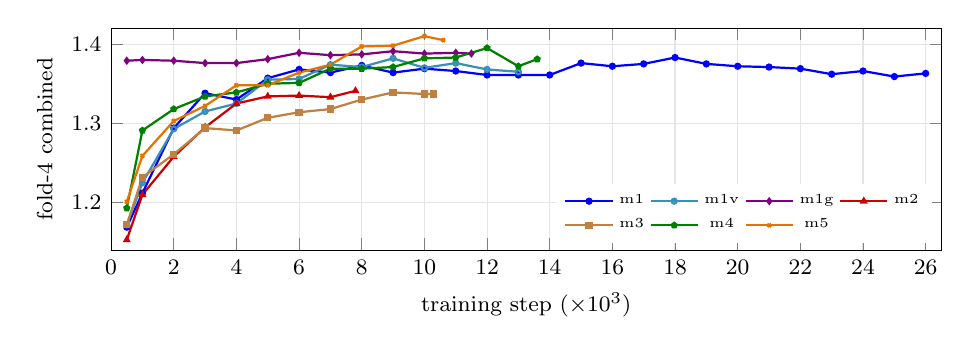
\begin{tikzpicture}
\begin{axis}[width=\columnwidth, height=4.4cm, xlabel={training step ($\times10^3$)},
  ylabel={fold-4 combined}, xmin=0, xmax=26.5, ymin=1.14, ymax=1.42, grid=major, grid style={gray!20},
  font=\footnotesize, yticklabel style={/pgf/number format/fixed, /pgf/number format/precision=2},
  legend style={font=\tiny, at={(0.99,0.03)}, anchor=south east, draw=none}, legend columns=4, every axis plot/.append style={thick, mark size=0.9pt}]
\addplot[blue, mark=*] coordinates {(0.5,1.169) (1.0,1.212) (2.0,1.294) (3.0,1.338) (4.0,1.330) (5.0,1.357)
  (6.0,1.368) (7.0,1.364) (8.0,1.373) (9.0,1.364) (10.0,1.369) (11.0,1.366) (12.0,1.361) (13.0,1.361) (14.0,1.361)
  (15.0,1.376) (16.0,1.372) (17.0,1.375) (18.0,1.383) (19.0,1.375) (20.0,1.372) (21.0,1.371) (22.0,1.369)
  (23.0,1.362) (24.0,1.366) (25.0,1.359) (26.0,1.363)};
\addlegendentry{m1}
\addplot[cyan!70!black, mark=o] coordinates {(0.5,1.172) (1.0,1.225) (2.0,1.293) (3.0,1.315) (4.0,1.325)
  (5.0,1.355) (6.0,1.356) (7.0,1.374) (8.0,1.371) (9.0,1.382) (10.0,1.370) (11.0,1.376) (12.0,1.368) (13.0,1.365)};
\addlegendentry{m1v}
\addplot[violet, mark=diamond*] coordinates {(0.5,1.379) (1.0,1.380) (2.0,1.379) (3.0,1.376) (4.0,1.376)
  (5.0,1.381) (6.0,1.389) (7.0,1.386) (8.0,1.387) (9.0,1.391) (10.0,1.388) (11.0,1.389) (11.5,1.388)};
\addlegendentry{m1g}
\addplot[red!80!black, mark=triangle*] coordinates {(0.5,1.153) (1.0,1.210) (2.0,1.258) (3.0,1.295) (4.0,1.325)
  (5.0,1.334) (6.0,1.335) (7.0,1.333) (7.8,1.341)};
\addlegendentry{m2}
\addplot[brown, mark=square*] coordinates {(0.5,1.172) (1.0,1.232) (2.0,1.261) (3.0,1.294) (4.0,1.291) (5.0,1.307)
  (6.0,1.314) (7.0,1.318) (8.0,1.330) (9.0,1.339) (10.0,1.337) (10.3,1.337)};
\addlegendentry{m3}
\addplot[green!50!black, mark=pentagon*] coordinates {(0.5,1.193) (1.0,1.291) (2.0,1.318) (3.0,1.334) (4.0,1.339)
  (5.0,1.350) (6.0,1.351) (7.0,1.369) (8.0,1.369) (9.0,1.371) (10.0,1.382) (11.0,1.383) (12.0,1.395) (13.0,1.372)
  (13.6,1.381)};
\addlegendentry{m4}
\addplot[orange!90!black, mark=x] coordinates {(0.5,1.201) (1.0,1.259) (2.0,1.303) (3.0,1.322) (4.0,1.348)
  (5.0,1.348) (6.0,1.364) (7.0,1.374) (8.0,1.397) (9.0,1.398) (10.0,1.410) (10.6,1.405)};
\addlegendentry{m5}
\end{axis}
\end{tikzpicture}
\caption{Fold-4 monitor score (best of student/EMA) during training, from the training logs, for the seven
members trained on our cluster (names as in Table~\ref{tab:members}; m1g continues from m1). Each released checkpoint is the step with the best monitor score.}
\label{fig:curves}
\end{figure}

\subsection{Snippet bank}
Subtracting clean from noisy audio at the labelled spans of the 695 validation synthetic pairs isolates 2,213
events, which deduplicate to \textbf{206 distinct snippets}. For every snippet, normalised cross-correlation (NCC)
is computed against each clip via FFT, keeping up to three peaks with $\text{NCC}\geq0.35$; edge sub-templates
(first or last 250\,ms) catch events truncated by the clip boundary. Each candidate is described by its NCC, a
\emph{chunk-lag consistency} score (whether every 50\,ms chunk peaks at the same lag, a property of sample-exact
copies but not of natural look-alikes), the implied SNR, the snippet duration and an edge flag. A logistic model
calibrated leave-fold-out maps these to a match probability, and greedy non-maximum suppression yields the bank
events.

\subsection{Fusion, routing and decoding}
Member caches are fused in the logit domain with the weights of Table~\ref{tab:members} (configuration
\texttt{clean\_plus\_a30}: 70\% on the six members trained without validation natural clips, 5\% on each of the
other six). The highest calibrated bank probability per clip (its \emph{synthetic score}) selects one of three
paths: \emph{bank}, where bank events above 0.56 confidence are merged with neural events above 0.64 (margin 0.18,
gap 200\,ms, at most five events); \emph{natural}, a category-aware hysteresis decoder (thresholds 0.85/0.61, median
filter of 5 frames, minimum 40\,ms, merge gap 160\,ms, boundary padding $-20/-30$\,ms) that splits blobs whose
category tracks disagree, so overlapping events of different types become separate events; and \emph{prior}, a
fallback so that no clip is left empty. All thresholds and fusion weights are searched with Optuna
TPE~\cite{optuna} on validation, with synthetic clips weighted $\times1.57$ to match the test mixture of 2,080
synthetic and 3,437 natural clips; the tuner reports a 5-fold CV estimate next to the full-validation score.

\section{Results and Conclusion}
\begin{table}[t]
\centering
\caption{Combined score (event F1 + segment Dice) on validation and on the Codabench test set for our Phase~1
entry and every Phase~2 submission. Validation scores of ensembles with validation-trained members include their
training folds; fold~4 is held out.}
\label{tab:res}
\footnotesize
\setlength{\tabcolsep}{3pt}
\begin{tabular}{llccc}
\toprule
ID & Configuration & Val.\ (2,501) & Fold 4 (479) & Test\\
\midrule
938975 & \texttt{s9000}+\texttt{s1600} (Phase 1) & 1.134 & -- & 1.2129\\
995013 & interim, clean members & 1.468 & 1.466 & 1.5803\\
995109 & all 12, fold-4 tuned, test-mix & 1.541 & 1.512 & 1.5854\\
995114 & all 12, fold-4 tuned & 1.541 & 1.512 & 1.5857\\
995138 & clean members, test-mix & 1.482 & 1.465 & 1.5875\\
\textbf{995227} & \textbf{clean + 30\% others} & 1.533 & 1.480 & \textbf{1.5943}\\
\bottomrule
\end{tabular}
\end{table}

\begin{table}[t]
\centering
\caption{Final configuration on validation by clip type (test-mix weighting). The bank's snippets come from the
synthetic validation clips themselves, so their synthetic score is an in-sample upper bound.}
\label{tab:split}
\footnotesize
\setlength{\tabcolsep}{4pt}
\begin{tabular}{lcccc}
\toprule
Subset & Clips & Event F1 & Seg.\ Dice & Combined\\
\midrule
Natural & 1,806 & 0.429 & 0.721 & 1.150\\
Synthetic (in-sample bank) & 695 & 0.999 & 0.996 & 1.995\\
All, test-mix weighted & 2,501 & 0.749 & 0.824 & 1.574\\
\midrule
\multicolumn{5}{l}{5-fold CV of the full configuration: 1.572 $\pm$ 0.021 (mean $\pm$ std)}\\
\bottomrule
\end{tabular}
\end{table}

\begin{figure}[t]
\centering
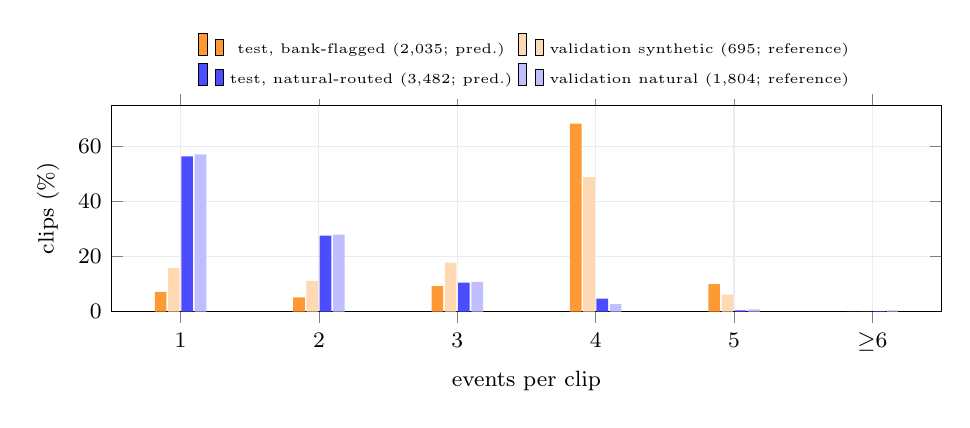
\begin{tikzpicture}
\begin{axis}[width=\columnwidth, height=4.2cm, ybar=0.6pt, bar width=4.2pt, xlabel={events per clip},
  ylabel={clips (\%)}, xtick={1,...,6}, xticklabels={1,2,3,4,5,$\geq$6}, ymin=0, ymax=75, font=\footnotesize,
  grid=major, grid style={gray!15}, enlarge x limits=0.1,
  legend style={font=\tiny, at={(0.5,1.03)}, anchor=south, draw=none}, legend columns=2]
\addplot[fill=orange!80, draw=none] coordinates {(1,7.2) (2,5.2) (3,9.3) (4,68.4) (5,10.0) (6,0.0)};
\addlegendentry{test, bank-flagged (2,035; pred.)}
\addplot[fill=orange!30, draw=none] coordinates {(1,15.8) (2,11.2) (3,17.8) (4,48.9) (5,6.2) (6,0.0)};
\addlegendentry{validation synthetic (695; reference)}
\addplot[fill=blue!70, draw=none] coordinates {(1,56.5) (2,27.6) (3,10.5) (4,4.7) (5,0.4) (6,0.2)};
\addlegendentry{test, natural-routed (3,482; pred.)}
\addplot[fill=blue!25, draw=none] coordinates {(1,57.2) (2,28.0) (3,10.8) (4,2.7) (5,0.8) (6,0.4)};
\addlegendentry{validation natural (1,804; reference)}
\end{axis}
\end{tikzpicture}
\caption{Events per clip in our final test predictions, split by bank flag, against the validation reference
annotations. Natural-routed test predictions closely follow the natural reference distribution.}
\label{fig:hist}
\end{figure}

Tables~\ref{tab:res}--\ref{tab:split} and Fig.~\ref{fig:hist} summarise the results.
\begin{itemize}
\item \textbf{Final entry (995227):} event F1 0.7711 and segment Dice 0.8232 on the 5,517 test clips, combined
1.5943. It routes 1,974 clips through the bank (the test set has 2,080 synthetic clips), 3,482 through the natural
decoder and 61 through the prior, emitting 13,268 events.
\item \textbf{The bank transfers to the test set.} Event F1 rose from 0.47 for our Phase~1 entry to 0.77.
\item \textbf{Natural clips are the hard half.} On validation, natural clips reach only 1.150 combined
(Table~\ref{tab:split}); single members reach 1.34--1.41 on fold~4 (Table~\ref{tab:members}), and fusion lifts
the ensemble to 1.48 there.
\item \textbf{Members trained without validation natural clips generalise best.} \texttt{clean\_full\_tm} scores
lower than \texttt{final\_f4\_tm} on validation but higher on test; re-adding the other members at 30\% total weight
gave the best test score.
\item \textbf{Category-aware decoding matters.} About 30\% of consecutive natural event pairs overlap; splitting
fused blobs by category track recovers them as separate events.
\end{itemize}

\textbf{Novelty.} (i) Calibrated, consistency-checked matched filtering that exploits the reuse structure of the
synthetic mixtures; (ii) a generator that reproduces the organizers' mixtures with sample-exact labels for training;
(iii) a heterogeneous ensemble over five pretrained encoders, fused in logits under a held-out-aware weighting; and
(iv) test-mixture-weighted decoder tuning with routing.

\textbf{Conclusion.} Heterogeneous pretrained SED members combined with an explicit model of how the synthetic data
was built give a strong, well-calibrated detector. Natural clips remain the harder half; better boundary modelling
of overlapping natural events is the main avenue for improvement.

\bibliographystyle{IEEEtran}
\begin{thebibliography}{10}\setlength{\itemsep}{0pt}\footnotesize
\bibitem{vaani} S.~Pulikodan \emph{et~al.}, ``VAANI: Capturing the language landscape for an inclusive digital India,'' arXiv:2603.28714, 2026.
\bibitem{pretrainedsed} F.~Schmid, T.~Morocutti, F.~Foscarin, J.~Schl\"uter, P.~Primus, and G.~Widmer, ``Effective pre-training of audio transformers for sound event detection,'' in \emph{Proc. ICASSP}, 2025.
\bibitem{atst} X.~Li, N.~Shao, and X.~Li, ``Self-supervised audio teacher-student transformer for both clip-level and frame-level tasks,'' \emph{IEEE/ACM TASLP}, 2024.
\bibitem{beats} S.~Chen \emph{et~al.}, ``BEATs: Audio pre-training with acoustic tokenizers,'' in \emph{Proc. ICML}, 2023.
\bibitem{wavlm} S.~Chen \emph{et~al.}, ``WavLM: Large-scale self-supervised pre-training for full stack speech processing,'' \emph{IEEE JSTSP}, 2022.
\bibitem{w2vbert} Seamless Communication \emph{et~al.}, ``Seamless: Multilingual expressive and streaming speech translation,'' arXiv:2312.05187, 2023.
\bibitem{filteraug} H.~Nam, S.-H.~Kim, and Y.-H.~Park, ``FilterAugment: An acoustic environmental data augmentation method,'' in \emph{Proc. ICASSP}, 2022.
\bibitem{meanteacher} A.~Tarvainen and H.~Valpola, ``Mean teachers are better role models,'' in \emph{Proc. NeurIPS}, 2017.
\bibitem{optuna} T.~Akiba \emph{et~al.}, ``Optuna: A next-generation hyperparameter optimization framework,'' in \emph{Proc. KDD}, 2019.
\bibitem{metrics} A.~Mesaros, T.~Heittola, and T.~Virtanen, ``Metrics for polyphonic sound event detection,'' \emph{Applied Sciences}, vol.~6, 2016.
\end{thebibliography}

\end{document}
